\documentclass[12pt, twocolumn]{article}
\usepackage[utf8]{inputenc}

\usepackage{graphicx}
\usepackage{amsmath}
\usepackage{url}
\usepackage[backend=biber, style=numeric, sorting=ynt]{biblatex}
\bibliography{bibl}

\title{ODE representation - Square root}
\author{Julie Thiim Gadeberg \\ $201604903$}
\date{March 2019}

\begin{document}

\maketitle

\section{Introduction}

In this report we seek to create an algorithm that is capable of calculating the square root of any given real positive number $x$. The chosen programming language for the algorithm is C, and the algorithm is based on functions~(\cite{gsl}) from GNU Scientific Library that can solve the ordinary differential equations. This report firstly gives a short description of the created algorithm in section~\ref{sec:algorithm}, while a presentation of the results is given in section~\ref{sec:results}.

\section{The algorithm} \label{sec:algorithm}

We use the ODE representation given by:
\begin{equation}
    \frac{\textup{d}y}{\textup{d}x} = \frac{1}{2y},
\end{equation}
as a starting point in order to calculate the square root of $x$. The first part of the algorithm is to define this equation in a separate function that depends on the variables $x$ and $y$, as well as the value of the equation parameters. The function stores the solution in the defined array $dydx$, while returning the message \texttt{GSL\_SUCCESS}.

Afterwards, it is possible to set up the function that solves the ODE. The function only takes $x$ as an input, but i order to avoid complex numbers, it is asserted that the given $x$ value is larger than or equal to zero. If this is not the case an error occurs, and the program terminates. The range of the argument is also reduced using the formula:
\begin{align}
    \frac{1}{\sqrt{\frac{1}{x}}} \hspace{5pt} &\textrm{if} \hspace{5pt} x < 1\\
    2\sqrt{\frac{x}{4}} \hspace{5pt} &\textrm{if} \hspace{5pt} x > 4.
\end{align}

Once the range is appropriate, we proceed to define the system of equations by using \texttt{gsl\_odeiv2\_system} as the data type, and combine it with the equation function. The problem is one-dimensional, and no parameters need to be defined, as the ODE does not include any such parameters. Afterwards, a driver  combining the steps, control, and evolution of the ODE system is chosen. We choose to use the \texttt{gsl\_odeiv2\_driver}. It takes the chosen data type, step type (\texttt{gsl\_odeiv2\_step\_rk8pd}), step size, absolute and relative precision as arguments. The driver is then applied stepping from the initial value of $x$ to the given $x$ argument. The result is stored in the given vector $y$ that is returned from this function, but if an error occurs an error message indicating the error type is returned instead. However, before returning either results, the driver is freed from the memory.

The last part of the algorithm is the main function. This function only includes a for loop that prints the variable $x$, the ODE solution and the value obtained from the \texttt{<math.h>} library. 


\section{Results} \label{sec:results}

For our purposes we let $x$ range from $0$ to $25$ with $\Delta x = 0.2$. The given initial condition is $y(1) = 1$, and the result is seen in figure~\ref{fig:sqrt}. 
\begin{figure}[ht]
    \centering
    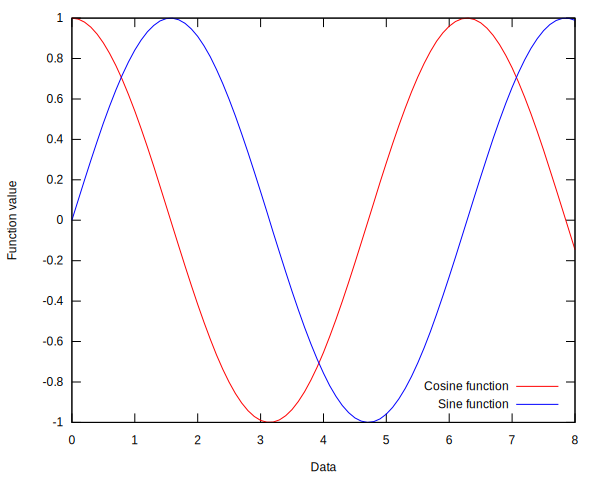
\includegraphics[width=\columnwidth]{plot.pdf}
    \caption{A plot of the results from the created algorithm and the square root function from the \texttt{<math.h>} library in black and grey respectively. The abscissa shows the different values of $x$, while the ordinate shows the corresponding value of $y$}
    \label{fig:sqrt}
\end{figure}
The figure depicts the results of the created algorithm, and the corresponding function from the \texttt{<math.h>} library. It is clear that the created algorithm works as intended as both of the functions are in agreement. 

\printbibliography

\end{document}
